\documentclass{standalone}
\usepackage{tikz}
\usepackage{pgfmath}
\usetikzlibrary{positioning}
\usetikzlibrary{calc}

\begin{document}
    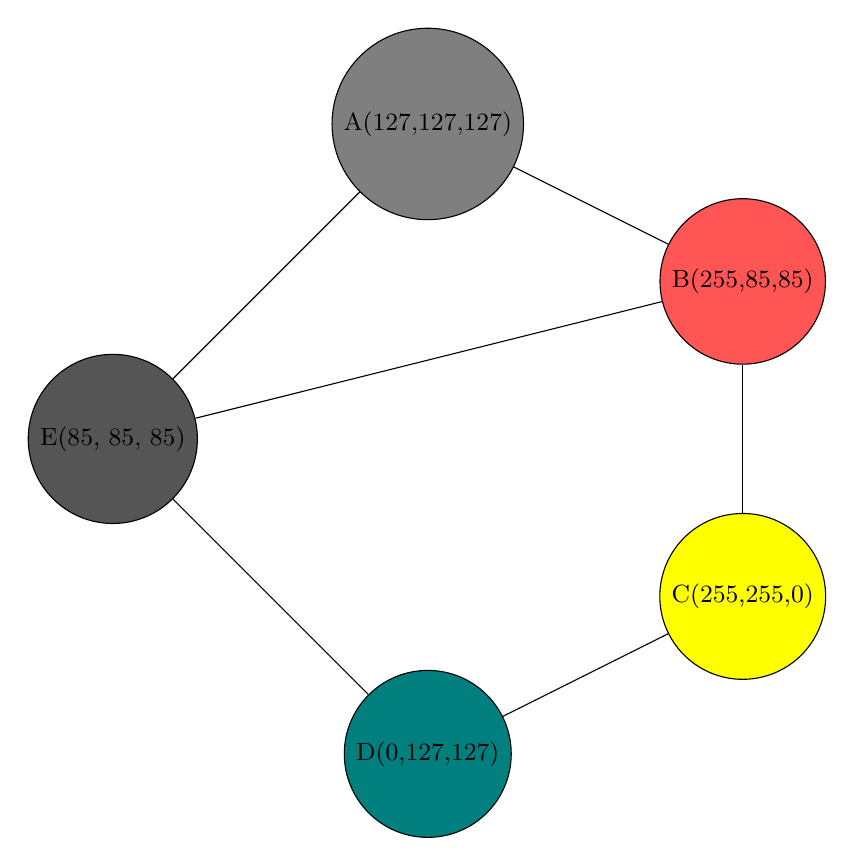
\begin{tikzpicture}[
        scale=1, 
        every node/.style={circle, draw, minimum size=2cm},
    ]
        \definecolor{Afinal}{RGB}{127,127,127}
        \definecolor{Bfinal}{RGB}{255,85,85}
        \definecolor{Cfinal}{RGB}{255,255,0}
        \definecolor{Dfinal}{RGB}{0,127,127}
        \definecolor{Efinal}{RGB}{85,85,85}

        % Final State
        \begin{scope}[xshift=12cm, local bounding box=finalstate]
        \node[fill=Afinal] (A) at (0,4) {\small{A(127,127,127)}};
        \node[fill=Bfinal] (B) at (4,2) {\small{B(255,85,85)}};
        \node[fill=Cfinal] (C) at (4,-2) {\small{C(255,255,0)}};
        \node[fill=Dfinal] (D) at (0,-4) {\small{D(0,127,127)}};
        \node[fill=Efinal] (E) at (-4,0) {\small{E(85, 85, 85)}};

        % Edges
        \draw (A) -- (B);
        \draw (A) -- (E);
        \draw (B) -- (C);
        \draw (C) -- (D);
        \draw (D) -- (E);
        \draw (B) -- (E);

        \end{scope}
    \end{tikzpicture}

\end{document}